\documentclass[a4paper,12pt]{article}

\usepackage[14pt]{extsizes}
\usepackage{cmap}					% поиск в PDF
\usepackage{mathtext} 				% русские буквы в формулах
\usepackage[T2A]{fontenc}			% кодировка
\usepackage[utf8]{inputenc}			% кодировка исходного текста
\usepackage[english,russian]{babel}	% локализация и переносы
\usepackage{graphicx}
\usepackage{geometry}
\usepackage{amsmath}
\usepackage{amssymb}
\usepackage[table]{xcolor}
\usepackage{multirow}


\geometry{verbose, a4paper, tmargin=2cm, bmargin=2cm, lmargin=3cm, rmargin=2cm}
\author{Vysotsky Maxim}
\title{Отчёт}
\date{2022}

\begin{document}
	\begin{titlepage}
		\begin{center}
			{Министерство науки и высшего образования Российской Федерации
				НОВОСИБИРСКИЙ НАЦИОНАЛЬНЫЙ ИССЛЕДОВАТЕЛЬСКИЙ
				ГОСУДАРСТВЕННЫЙ УНИВЕРСИТЕТ (НГУ)}
		\end{center}
		\begin{center}
			{Физический факультет}
		\end{center}
		\begin{center}
			{Кафедра общей физики}
		\end{center}
		
		
		\vspace{7cm}
		{
			\begin{center}
				{\bf Лабораторная работа №2.1}\\
				Электроизмерительные приборы и источники питания постоянного
тока
			\end{center}
		}
		\vspace{2cm}
		\begin{flushright}
			{Руководитель:\\ Старший преподаватель\\
				Яцких А. А.\\
				Работу выполнил:\\
				Высоцкий М. Ю.\\
				\vspace{0.2cm}
				гр. 24301}
		\end{flushright}
		\vspace{3cm}
		\begin{center}
			Новосибирск, 2024
		\end{center}
	\end{titlepage}

\section{Теоретическое введение}
\textbf{Цель работы:} Познакомиться с устройством, принципом действия электромеханических и цифровых измерительных приборов; научиться проводить измерения тока и напряжения в цепях постоянного тока, а также с режимами работы источников питания постоянного тока.

\textbf{Оборудование:} Источники питания постоянного тока, вольтметры, амперметры, цифровые мультиметры, магазин сопротивлений, макетные платы.

\section{Ход работы.}
\subsection{Задание 1. Изучение влияния вольтметра на режим работы
электрической цепи постоянного тока.}

\hspace{\parindent}В данном задании требуется измерить разность потенциалов на клеммах источника тока и сравнить ее со значением, полученным при измерении разности потенциалов в точках А и В. Для этого к соответствующим точкам надо было подключить мультиметр, переведенный в режим измерения постоянного напряжения (DC, V). Также требовалось посчитать сопротивление на $R_2$. Схема установки приведена ниже.

\begin{figure}[h!]
	\begin{center}
		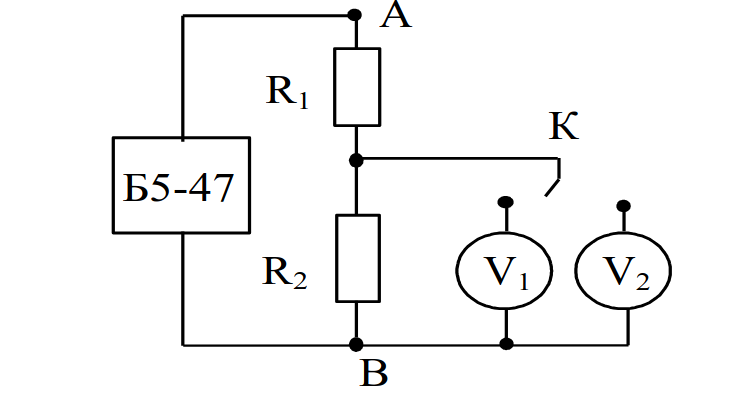
\includegraphics[scale=0.6]{scheme_1.png}
	\end{center}
	\caption{Электрическая схема задания 1.}
\end{figure}
Здесь \textbf{V1} - вольтметр М2044, \textbf{V2} - вольтметр GDM-8145.

Показания, снятые во время опыта:

\begin{table}[h!]
    \centering
    \begin{tabular}{|l|l|l|}
        \hline
        $R_{1-2}$, кОм & $R_1$, кОм & $R_2$, кОм \\ \hline
        300 & 148,63 & 152,75 \\ \hline
    \end{tabular}
\end{table}

Показания напряжения на источнике и на сопротивлении: $U_{ист}$ = 20.0 В, $U_{AB}$ = 19,99 В.

\newpage

Формула для поиска напряжения на 2-м сопротивлении.
\begin{equation}
    U_2 = \frac{R_2}{R_1+R_2}U_{AB}
\end{equation}
Согласно формуле, $U_2$ = 10,131 В.

Теоретическое напряжение рассчитывается по формуле распределения
напряжений с учетом того, как считается напряжение при параллельном
соединении:
\begin{equation}\label{u_teor}
    U_{теор} = \frac{R_2 R_V}{R_V(R_1+R_2)+R_1R_2}U_{AB}
\end{equation}

Исходя из данных, сопротивление источника $R_{ист} = \frac{U_{ист}}{I_{ист}} = \frac{20}{0,1} = 200$ Ом.

С учётом наличия теоретического сопротивления, (\ref{u_teor}) будет выглядеть следующим образом:
\begin{equation}\label{u_teor_ist}
    U_{теор} = \frac{R_2 R_V}{R_V(R_1+R_2+R_{ист})+(R_1+R_{ист})R_2}U_{AB}
\end{equation}

Итого, таблица по данному заданию:
\begin{table}[!ht]
    \centering
    \begin{tabular}{|l|l|l|l|l|l|l|l|}
    \hline
        Вольметр & Шкала, В & U, В & $U_{теор}$, В & Rv, Ом & \multicolumn{2}{l|}{U, В ( пар. с.)} \\ \hline
        GDM & 20 & $10,043\pm0,007$ & 10,049 & $10^7$   & GDM   & M2044 \\ \hline
        M2044 & 75 & $8,50\pm0,15$  & 8,798 & $5*10^5$ & 8,74 & 8,5 \\ \hline
        M2044 & 30 & $4,00\pm0,06$  & 4,04 & $5*10^4$ & 4,03  & 4,0 \\ \hline
        M2044 & 15 & $4,00\pm0,03$  & 4,04 & $5*10^4$ & 4,03  & 4,0 \\ \hline
    \end{tabular}
\end{table}

\subsection{Вывод по заданию.}
Причиной различия показаний вольтметров является сопротивление 
вольтметра: чем меньше $R_V$, тем больше отличие измеренных показаний от расчётных. Поэтому главное требование для вольтметра: $R_V \xrightarrow{} \infty$.

\newpage

\subsection{Задание 2. Изучение влияния амперметра на режим работы
электрической цепи постоянного тока.}

\hspace{\parindent}Для выполнения задания необходимо измерить величину
сопротивления R, установить на источнике напряжение 0,1 В, ток 0,1 А,
установить на мультиметре режим измерения постоянного тока и предел
измерения 200 мА. Записать значения
силы тока указав погрешности и провести измерения на пределах измерения
20 и 2 мА. Схема приведена ниже.

\begin{figure}[h!]
	\begin{center}
		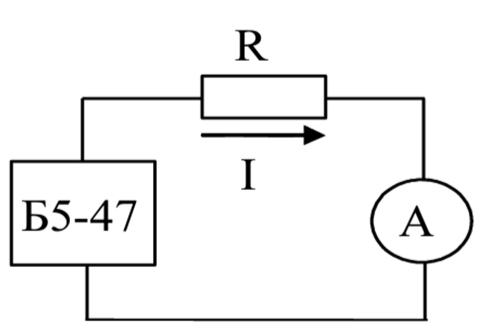
\includegraphics[scale=0.8]{scheme_2.png}
	\end{center}
	\caption{Электрическая схема задания 2.}
\end{figure}

Снятые показания: $U$ = 0,098 В, $R$= 10,5 Ом. 

Далее идёт таблица с показаниями. Сопротивления $R_A$ брались из паспорта. 

\begin{table}[!ht]
    \centering
    \begin{tabular}{|l|l|l|l|l|l|}
    \hline
        Предел, мА & $I_{эксп}$, мА & $\Delta I$ & $R_{а}$, Ом & $I_{R}$, мА (с $R_{a}$) & $I_R$, мА (без $R_a$) \\ \hline
        200 & 8 & 0,0116 & 2 & 7,84 & 9,3 \\ \hline
        20 & 4,67 & 0,0667 & 11,4 & 4,47 & ~ \\ \hline
        2 & 0,8 & 0,01 & 100,8 & 0,88 & ~ \\ \hline
    \end{tabular}
\end{table}

\subsection{Вывод по заданию.}
\hspace{\parindent}Чем выше сопротивление амперметра, тем меньше сила тока в цепи. Поэтому условие
идеального амперметра – нулевое сопротивление амперметра $R_A \xrightarrow{} 0$ 

\newpage

\subsection{Задание 3. Определение сопротивления электростатического
вольтметра.}

\hspace{\parindent}Для выполнения задания необходимо зарядить ёмкость
электростатического вольтметра любым известным методом и записывать
изменение показаний вольтметра через некоторые интервалы времени в
течение 40 минут. Результаты занести в таблицу, построить график
зависимости от времени $\ln(\frac{U}{U_0})$ и по угловому коэффициенту определить
сопротивление вольтметра.

Начальное напряжение было равно: $U_0$ = 52 В.

\begin{table}[!ht]
    \centering
    \begin{tabular}{|l|l|l|}
    \hline
        t, с & U, В & $lnU/U_0$ \\ \hline
        100 & 70 & 0 \\ \hline
        450 & 65 & -0,07 \\ \hline
        1080 & 60 & -0,15 \\ \hline
        1660 & 52 & -0,3 \\ \hline
        1800 & 51 & -0,32 \\ \hline
        1950 & 50 & -0,34 \\ \hline
        2160 & 49 & -0,36 \\ \hline
        2380 & 48 & -0,38 \\ \hline
    \end{tabular}
\end{table}

И получили график:

\begin{figure}[h!]
	\begin{center}
		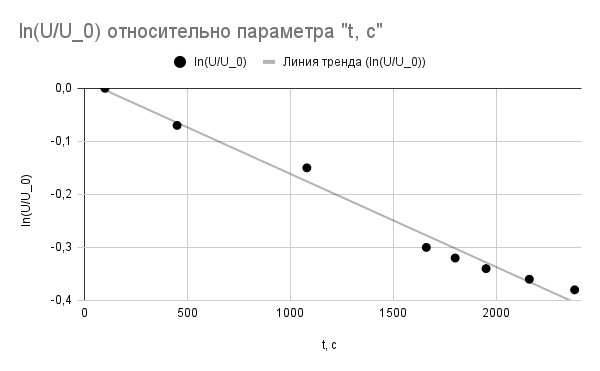
\includegraphics[scale=0.6]{ln.png}
	\end{center}
	\caption{Зависимость $\ln U/U_0(t)$}
\end{figure}

Коэффициент наклона прямой равен $k$ = -0,0002.

Продифференцировав $\ln(\frac{U}{U_0})$ по времени получим следующую зависимость:

\begin{equation}
    R = -\frac{1}{kC}
\end{equation}

Из паспортных данных вольтметра узнаем значение емкости $C$ = $10^{-11}$Ф, подставим
в формулу и определим значение сопротивления.
Оно будет равно $R\approx 5*10^{14}$ Ом.

\subsection{Вывод по заданию.}
\hspace{\parindent}Из графика (как логарифмического, как и не логарифмического) видно, что напряжение падает практически линейно.

\subsection{Задание 4. Определение ЭДС и внутреннего сопротивления источника}
\hspace{\parindent}Для выполнения задания предлагается собрать схему, на
мультиметре установить режим измерения постоянного напряжения с
пределом измерения 200 В, а для магнитоэлектрического прибора на двух
пределах: 75 и 150 В. По полученным данным определить ЭДС и внутреннее
сопротивление источника тока.

\begin{figure}[h!]
	\begin{center}
		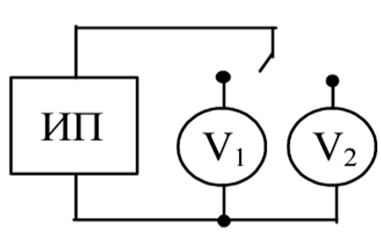
\includegraphics[scale=0.8]{scheme_4.png}
	\end{center}
	\caption{Электрическая схема задания 4.}
\end{figure}

Ниже преведены данные.
\begin{table}[!ht]
    \centering
    \begin{tabular}{|l|l|l|l|l|}
    \hline
        V & Шкала, В & U, в & $\Delta U$, Ом  & $R_V$ Ом \\ \hline
        GDM & 200 & 66,82 & 0,04 & $10^7$ \\ \hline
        M2044 & 150 & 48,3 & 0,2 & $10^6$ \\ \hline
        M2044 & 75 & 37 & 0,2 & $5*10^5$ \\ \hline
    \end{tabular}
\end{table}

Составим систему и решим её:
\begin{equation}
    \begin{cases}
    \mathcal{E}_i = I_i(R_i + r)\\
    I_iR_i=U_i
    \end{cases}
\end{equation}

Решая попарно 1 и 2, 2 и 3, 3 и 1, получим:

\begin{equation}
    \begin{cases}
    \mathcal{E} = 66,82 * (1+\frac{r}{10^7})\\
    \mathcal{E} = 48,3 * (1+\frac{r}{10^6})\\
    \mathcal{E} = 37 * (1+\frac{r}{5*10^5})\\
    \end{cases}
\end{equation}
Из 1 и 2: $\mathcal{E}$ = 69,79 В;\textbf{ r = 445000 }Ом\\
Поставим r в 1 и 2, получим: \\1: $\mathcal{E}$ = 69,79 В;\\ 2: $\mathcal{E}$ = 69,93 В. 

Получаем $\varepsilon \approx 69,84$ Ом.

\subsection{Вывод по заданию.}
\hspace{\parindent}Мы получили внутренее сопротивление источника $r$ = 445000 Ом и ЭДС $\mathcal{E}\approx 69,84$ В.

\subsection{Задание 5. Изучение работы стабилизированного
источника питания постоянного тока в режимах
стабилизации тока и стабилизации напряжения}

В задании предложено собрать схему, приведенную ниже. Меняя
сопротивление с шагом в 10 Ом на магазине сопротивлений, необходимо измерить
соответствующие значения напряжения и тока, а по полученным данным определить
величину сопротивления нагрузки, соответствующую смене режима стабилизации. Далее
было предложено построить графики зависимости тока, напряжения и выделяемой
мощности от сопротивления нагрузки.

\begin{figure}[h!]
	\begin{center}
		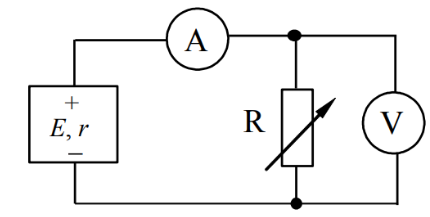
\includegraphics[scale=0.8]{scheme_5.png}
	\end{center}
	\caption{Электрическая схема задания 5.}
\end{figure}

\newpage
Данные приведены ниже:
\begin{table}[!ht]
    \centering
    \begin{tabular}{|l|l|l|l|}
    \hline
        R, Ом & U, В & I, мА & P, мВт \\ \hline
        99,9 & 11,905 & 120,07 & 1429,433 \\ \hline
        89,9 & 11,888 & 133,35 & 1585,265 \\ \hline
        79,9 & 11,867 & 149,93 & 1779,219 \\ \hline
        69,9 & 11,838 & 171,22 & 2026,902 \\ \hline
        59,9 & 11,987 & 203,3 & 2436,957 \\ \hline
        49,9 & 10,097 & 206,2 & 2082,001 \\ \hline
        39,9 & 8,069 & 207,2 & 1671,897 \\ \hline
        29,9 & 6,039 & 208,4 & 1258,528 \\ \hline
        19,9 & 3,968 & 209,2 & 830,106 \\ \hline
        9,9 & 1,883 & 209,9 & 395,242 \\ \hline
    \end{tabular}
\end{table}

Мощность расчитываем по следующей формуле:
\begin{equation}
    P = UI
\end{equation}

\begin{figure}[h!]
	\begin{center}
		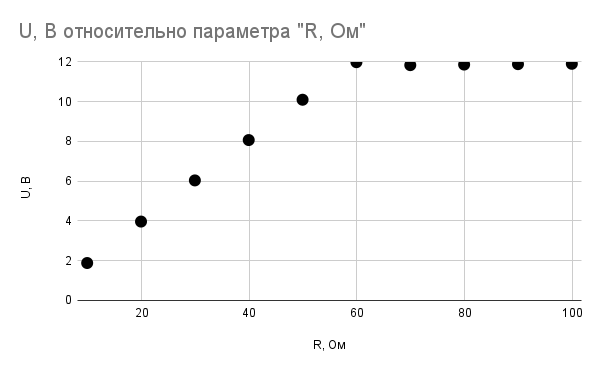
\includegraphics[scale=0.8]{ur1.png}
	\end{center}
\end{figure}
\newpage
\begin{figure}[h!]
	\begin{center}
		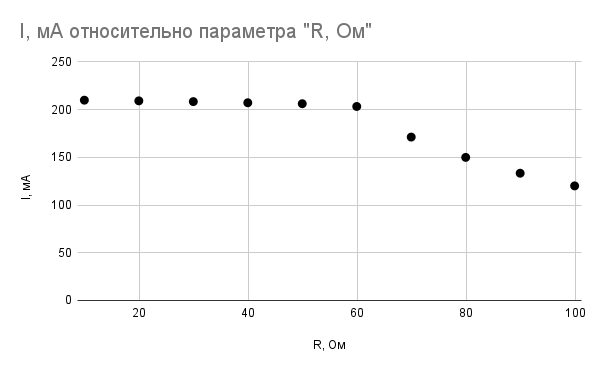
\includegraphics[scale=0.8]{ir.png}
	\end{center}
\end{figure}

\begin{figure}[ht!]
	\begin{center}
		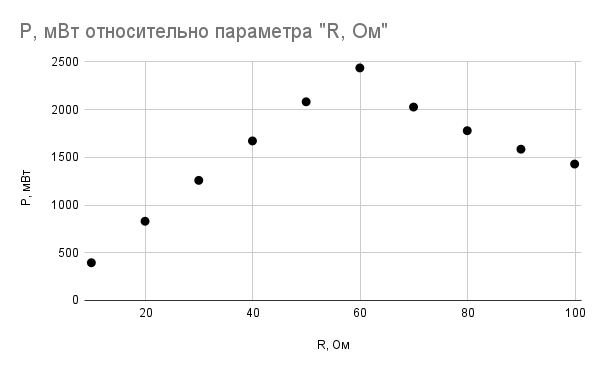
\includegraphics[scale=0.8]{pr.png}
	\end{center}
\end{figure}

Из последнего графика видно, что стабилизация происходит при R = 60 Ом.

\subsection{Вывод по заданию.}
Режиму стабилизации тока соответствует сопротивление нагрузки R<<r, т.к. падение
напряжения на нагрузке меняется пропорционально ее сопротивлению:
\begin{equation}
    I = \frac{\mathcal{E}}{r+R} \approx \frac{\mathcal{E}}{r} \approx const
\end{equation}

Режиму стабилизации напряжения соответствует сопротивление R>>r, в этом случае ток в
цепи обратно пропорционален сопротивлению нагрузки:
\begin{equation}
    I = \frac{\mathcal{E}}{r+R} \approx \frac{\mathcal{E}}{R} \approx const
\end{equation}
$U=IR\approx\mathcal{E}\approx const$ (напряжение на нагрузке не зависит от сопротивления нагрузки)

\section{Вывод по работе}
\begin{enumerate}
    \item Установлено требование к вольтметру: сопротивление вольтметра
должно быть на несколько намного меньше выше, чем измеряемое. Таким образом $R_V \xrightarrow{} \infty$.
    \item Установлено требование к амперметру: сопротивление амперметра
должно быть на несколько порядков ниже, чем измеряемое. Таким образом, $R_A \xrightarrow{} 0$ 
    \item Определена ёмкость электростатического вольтметра С-50:\\ $C$ = $10^{-11}$ Ф.
    \item Установлено ЭДС и сопротивление и источника.
    \item Изучена работа стабилизированного источника питания, найдено сопротивление, при котором источник переходит в режим стабилизации (R = 60 Ом)

\end{enumerate}

\end{document}